\documentclass[11pt,a4paper]{report}
\usepackage{hyperref} % for \url
\PassOptionsToPackage{hyphens}{url}\usepackage{hyperref}

% \\~\\ double new line
% images
\usepackage{graphicx} 
\usepackage{float}
\usepackage{polski}
\graphicspath{ {./images/} }

\usepackage{amsmath}

\usepackage[utf8]{inputenc}
\usepackage[margin=3.5cm]{geometry}

%% ########################################################
\begin{document}
\thispagestyle{empty}
\begin{center}

\includegraphics[width=\textwidth]{logo_AGH.jpg}\\
\bf{\sf{WYDZIAŁ FIZYKI I INFORMATYKI STOSOWANEJ}}\\[5mm]
%% ======================================================
\bf{\sf{KATEDRA ODDZIAŁYWAŃ I DETEKCJI CZĄSTEK}}\\[14mm]
%% ======================================================
\sf{\huge Praca dyplomowa}\\[12mm] 
%% ======================================================
\sf{\Large First application of the diffusion and transformer models for medical CT scans analysis in scope of MonAI platform \\[2mm] 
Pierwsze zastosowanie modeli dyfuzyjnych i modeli typu transformer do analizy medycznych skanów tomografii komputerowej w ramach platformy MonAI \\[2mm]
%% ======================================================
%% W przypadku pracy napisanej
%% - po polsku: dwa tytuły,
%% - po angielsku: dwa tytuły,
%% - po hiszpańsku/niemiecku/rosyjsku/etc: trzy tytuły.
%% ======================================================
}
\vspace{40mm}
\end{center}
\sf{
\begin{tabular}{l l}
Autor: & Piotr Harmuszkiewicz \\
Kierunek studiów: &	Informatyka Stosowana\\
Opiekun pracy: & prof. dr hab. inż. Tomasz Szumlak\\
\end{tabular}
}\\[10mm]
\begin{center}
\sf{Kraków, 2023}
\end{center}

%% ########################################################
\newpage
%% ########################################################

\subsubsection{Acknowledgement}
I would like to express gratitude to Zuzanna Harmuszkiewicz for providing me with valuable advice and insight on the topic of my thesis and for taking time to read and review my work.
\newpage
\tableofcontents
\chapter{Goals and motivation of the thesis.}
This graduation thesis aimed to develop a diffusion model able to generate new medical CT scans and perform quality analysis of obtained results. The motivation for the implementation of the project was solving the problem of insufficient amount of training data, required for different machine learning solutions used in medical field. 
The first chapter is an introduction to the study, explaining the goal and motivation of the project. 
Next chapter contains theoretical foundations, the chapter covers essential concepts like diffusion models and attention. 
In the third chapter the implementation of the project was explained, detailing the project environment, model architecture, training process and dataset.
The final chapter presents the outcomes, which are analyzed in terms of – visual quality, diversity, and are compared to original data. This chapter also presents limitations and conclusion.

\chapter{Theoretical Basis}

\section{Convolutional neural networks}
Convolutional neural networks (CCN) are type of neural network that are suited for grid-like data (e.g. images, which are two dimensional grid of pixels). CNNs use mathematical operation: convolution that combines two functions to produce third function. In machine learning we usually use kernel, which is small matrix. The kernel is moved along and across input data and applying kernel results in matrix, which is called feature map. The values of kernels are trainable neural network's parameters.
\cite{convolution} \cite{Michal}

\begin{figure}[H]
	\centering
	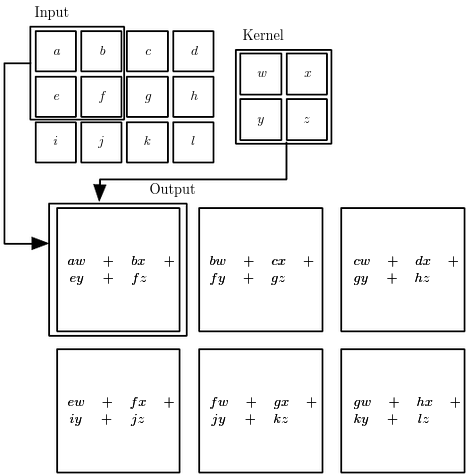
\includegraphics[scale=0.6]{images/convolution}
    \caption{Example of kernel and 2D convolution \cite{convolution}}
\end{figure} 

\section{Generative models}
Generative models are type of algorithms that aims to create new examples similar to data from dataset. Generative models learn probability distribution of training dataset and are able to generate complicated data based on this distribution.
\section{Diffusion models}
Diffusion models are type of generative models, that aims to model distribution of data from a given dataset. They use Markov chain, which represent sequence of steps in which small random noise is added to data and then model learns to gradually reverse diffusion steps. Diffusion model contains two components: forward diffusion process and reverse diffusion process.

\subsection{Forward diffusion process}
During forward diffusion process we define Markov chain with T steps, which are more and more noised samples from dataset. The result is sequence: $x_1,..., x_T$  of samples with distribution $q(x_t|x_{t-1})$:
\[ q(x_t|x_{t-1}) = N(x_t;\sqrt{1-\beta_t}x_{t-1}, \beta_tI) \]
\[ q(x_{1:T}|x_0) = \prod_{t=1}^{T}{q(x_t|x_{t-1})} \]

In each step we add small amount of Gaussian noise with the variance $\beta_t$. For $T\rightarrow\infty$, $x_T$ is isotropic Gaussian distribution, however for well-chosen values of $T$ and $\beta_1,..., \beta_T$ it is nearly an isotropic Gaussian distribution and is sufficient for diffusion models.

$\beta_t$ is constant increased with step $t$ according to variance schedule, linear function can be used e.g. $B_1=10^{-4}$, $B_T=0.02$ for $T=1000$. \cite{DDPM}

\begin{figure}[H]
	\centering
	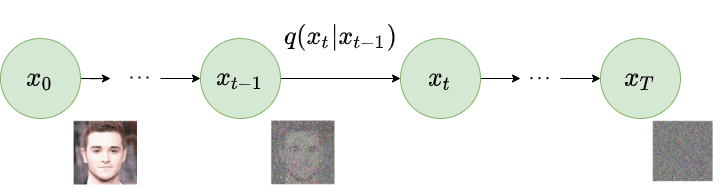
\includegraphics[width=\textwidth]{images/forward-diffusion}
    \caption{Example of Markov chain for image \cite{DDPM}}
\end{figure}

\subsection{Reparameterization trick}
The basic idea of the reparameterization trick is to express a random variable sampled from a certain distribution as a deterministic function of a separate random variable and a fixed parameter. This reparameterization allows for the separation of the randomness in the model from the gradient computations, which makes the optimization process more stable. Instead of directly sampling from the distribution (usually a Gaussian), we sample from a standard Gaussian distribution (mean=0, variance=1) and then transform this sample using the learned mean and variance parameters. 
Mathematically, we can denote the random variable as $z$ and its distribution as $q(z|x)$, the trick involves representing $z$ as:
\[z=\mu + \sigma \odot \epsilon,\]
where:
\begin{itemize}
\item $\mu$ - mean value learned by network 
\item $\sigma$ - standard deviation learned by network 
\item $\epsilon$ - sample from Gaussian distribution ($\epsilon \sim N(0,I)$)
\item $\odot$ - element-wise multiplication
\end{itemize}
Now we can rewrite formula for $q(x_t|x_{t-1})$ using reparameterization trick as:
\[q(x_t|x_{t-1}) = \sqrt{1 - \beta_t}x_{t-1} + \sqrt{\beta_t}\epsilon\]
Let $\alpha_t = 1 - \beta_t$, $\bar{\alpha}_t = \prod_{i=1}^{t}{\alpha_i}$, so:
\[q(x_t|x_{t-1}) = \sqrt{\alpha_t}x_{t-1} + \sqrt{1-\alpha_{t}}\epsilon\]
\[q(x_t|x_{t-2}) = \sqrt{\alpha_t \alpha_{t-1}}x_{t-2} + \sqrt{1-\alpha_t \alpha_{t-1}}\epsilon\]
\[q(x_t|x_0) = \sqrt{\bar{\alpha}_t}x_0 + \sqrt{1-\bar{\alpha}_t}\epsilon\]
To get nth element from Markov chain we do not need to apply Gaussian noise $n$ times, which is slow for bigger values of $n$. It is enough to use equation above. \cite{lw_diffusion}
\subsection{Reverse diffusion process}
The idea behind reverse diffusion process is to undo the forward process and remove noise that was added. The reverse process is  also a Markov chain but this time neural network calculates the next element. Let $p_\theta$ be a reverse process function, which is probability density function.
\[p_\theta(x_{0:T}) = p(x_T)\prod_{t=1}^{T}{p_\theta(x_{t-1}|x_t)})\]
\[p_\theta(x_{t-1}|x_t) = N(x_{t-1};\mu_\theta(x_t, t), \Sigma_\theta(x_t,t))\]
In our case variance is known so: $\Sigma_\theta(x_t,t)=\bar{\beta_t}$.

To train the network we need loss function, which is defined as negative log-likelihood: $-log(p_\theta(x_0))$. However it is not easily computable, because $p_\theta(x_0)$ depends on the whole Markov chain. The solution is to use variational lower bound of the function:
\[-log(p_\theta(x_0)) \le -log(p_\theta(x_0)) + D_{KL}(q(x_{1:T}|x_0)||p_\theta(x_{1:T}|x_0))\]
$D_{KL}$ is KL divergences. The equation can be simplified \cite{ImprovedDDPM} and it will result in loss function: $L=||\epsilon - \epsilon_\theta(x_t, t)||^2$, which is just mean square error of applied noise and predicted noise.

\begin{figure}[H]
	\centering
	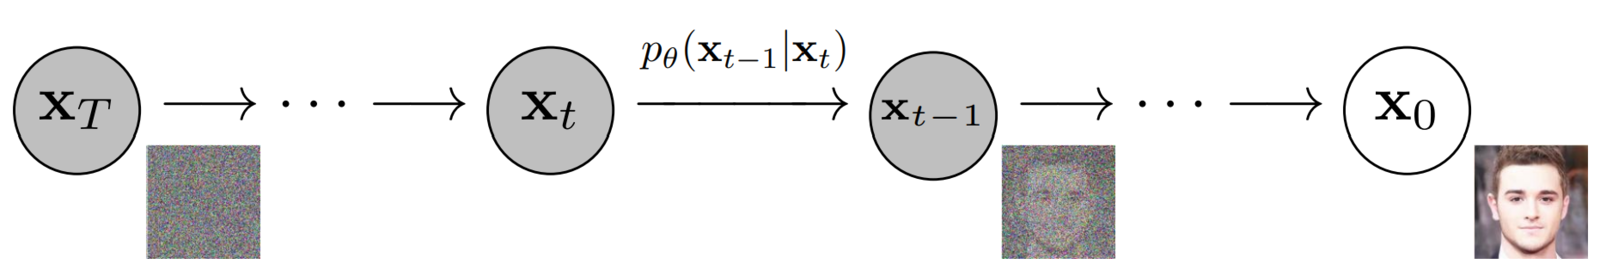
\includegraphics[width=\textwidth]{images/reverse-diffusion}
    \caption{Example of reverse diffusion process for image \cite{DDPM}}
\end{figure}

\section{Attention}
Attention, in the context of machine learning and natural language processing, is a mechanism that allows models to focus on specific parts of input data while making predictions or generating output. The concept of attention draws inspiration from human cognitive processes, where we naturally pay varying degrees of attention to different parts of information when processing it. Attention mechanisms are particularly useful in tasks where the model needs to consider different parts of input data with varying levels of importance or relevance.

\subsection{Attention block}
To use this mechanism we need to implement  an attention block. An attention block is a component in neural network architectures that implements an attention mechanism. It is one of the building blocks used in diffusion model. The attention block typically takes in a set of input representations and computes attention weights to emphasize the importance of different elements within the input. These elements could be words in a sentence, pixels in an image, or any other kind of structured data. The attention weights are then used to compute a weighted sum of the input representations, resulting in an enriched representation that captures contextual information and relationships between elements.

\begin{figure}[H]
	\centering
	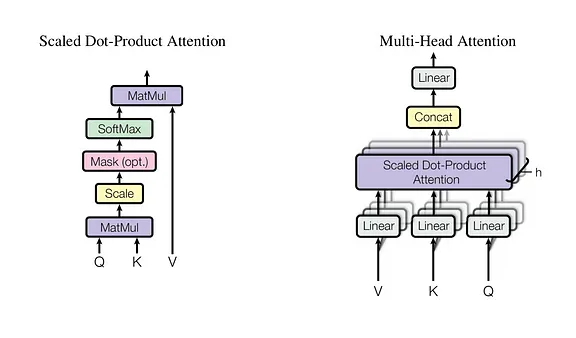
\includegraphics[width=\textwidth]{images/multi_headed}
    \caption{Mutli-Head Attention block \cite{AttentionIsAll}}
\end{figure}

Scaled dot-product attention can be describe with:
\[Attention(Q,K,V) = softmax(\frac{QK^T}{\sqrt{d_k}})V\]
Input of multi-headed attetion block is:
\begin{itemize}
\item query - represents the element that we are interested in understanding
\item key - holds information used to assess the importance of other elements
\item value - contains the actual content we want to focus on
\end{itemize}
All of these values are the same at the beginning.

In essence, the attention mechanism computes scores by comparing the query with keys. These scores reflect how much attention each element deserves. Then, these scores are used to blend the values together, forming an output representation that captures the essence of the input sequence. \cite{AttentionIsAll} \cite{AttentionWiki}\ cite{TransformersWiki}

\chapter{Implementation of the model}
This chapter will present the details of the project implementation: description of the development environment and the tools used during development. It will also describe dataset, implementation of the model and some details of selected aspects of the project.
\section{Project environment}
During development the following tools were used:
\begin{itemize}
\item Python 
\item PyTorch
\item Monai
\item Hugginface diffusers 
\end{itemize}
\subsection{Python}
Python is a high-level, and widely used programming language known for its simplicity, readability, and extensive libraries. In the context of machine learning, Python is popular due to its rich ecosystem of libraries, frameworks, and tools that make it easier to implement and experiment with various machine learning algorithms and techniques. \cite{Python}
\subsection{PyTorch}
PyTorch is an open-source machine learning framework that is used for developing and training machine learning models. PyTorch's central concept is the tensor, a multi-dimensional array, which is used for numerical computations and supports GPU acceleration for faster processing. The framework includes multiple tools to make it straightforward to design and build neural networks and has user-friendly API. \cite{Pytorch}
\subsection{Monai}
MONAI (Medical Open Network for AI) is an open-source framework built on PyTorch, designed exclusively for deep learning in medical imaging. It simplifies tasks like data handling, model creation, training, and deployment for medical image analysis. MONAI focuses on challenges unique to this domain, making it easier to develop and deploy AI models for tasks connected with healthcare. \cite{Monai}
\subsection{Huggingface diffusers}
Diffusers is an open-source library based on PyTorch. It offers framework for building UNet models and a lot of functionality used during training like noise scheduler. It also offers pre-trained networks and much more. The library is modular, which allows creating custom models and training pipelines. The library is easy to use and has good documentation. \cite{Hf_diffusers}
\subsection{Hardware}
Throughout the project, Nvidia Titan RTX GPU was used, equipped with 24GB of memory for the training and testing of networks. This GPU is compatible with CUDA, a platform that allows general-purpose computing on the GPU, and it is integrated into Pytorch. The primary constraint we encountered was related to memory limitations, primarily because of the extensive data.
\section{Implementation}
The source code is available at the link below:
\newline
\url{https://github.com/Harmek59/diffusion-ct}
\newline
Implementation of the model was base on the implementation of: UNet2DModel from diffusers library. The model was adapted to work with 3 dimensional data.
The model consists of few building blocks:
\begin{itemize}
\item Resnet
\item Attention
\item Downsample block
\item Upsample block
\item Midblock
\end{itemize}
\subsection{Resnet}
ResNet (Residual Network) is a type of neural network design for very deep architectures. It uses residual blocks that let the network learn and improve the difference between input and output. This makes training deep networks easier and helps avoid vanishing gradient problems. \cite{Resnet} Resnet block are the main building blocks of the network. They were proven to provide good results in image processing and are especially useful in deep networks.


\begin{figure}[H]
	\centering
	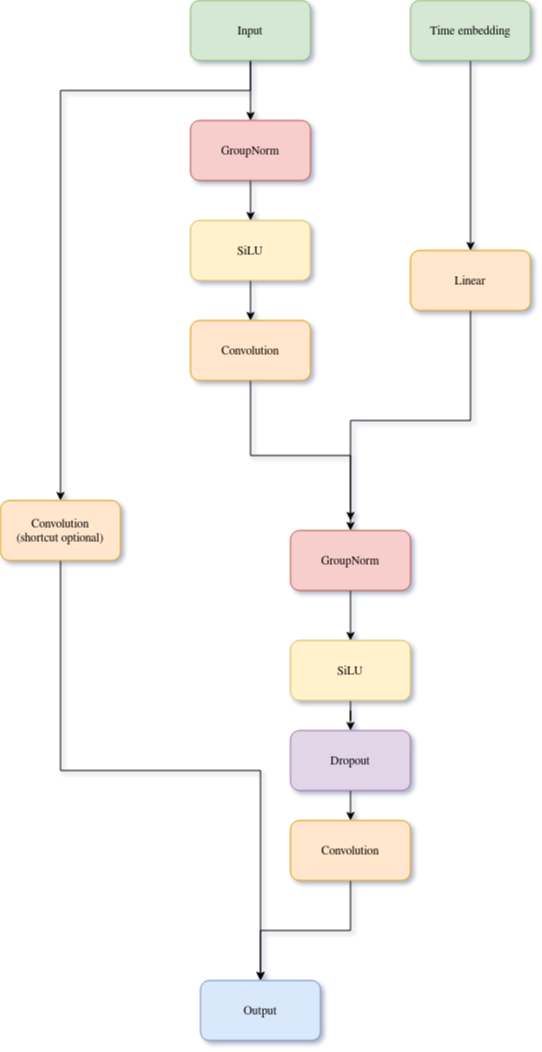
\includegraphics[scale=0.6]{images/ResnetBlock.drawio}
    \caption{Resnet block architecture diagram}
\end{figure}

\subsection{Attention block}
\begin{figure}[H]
	\centering
	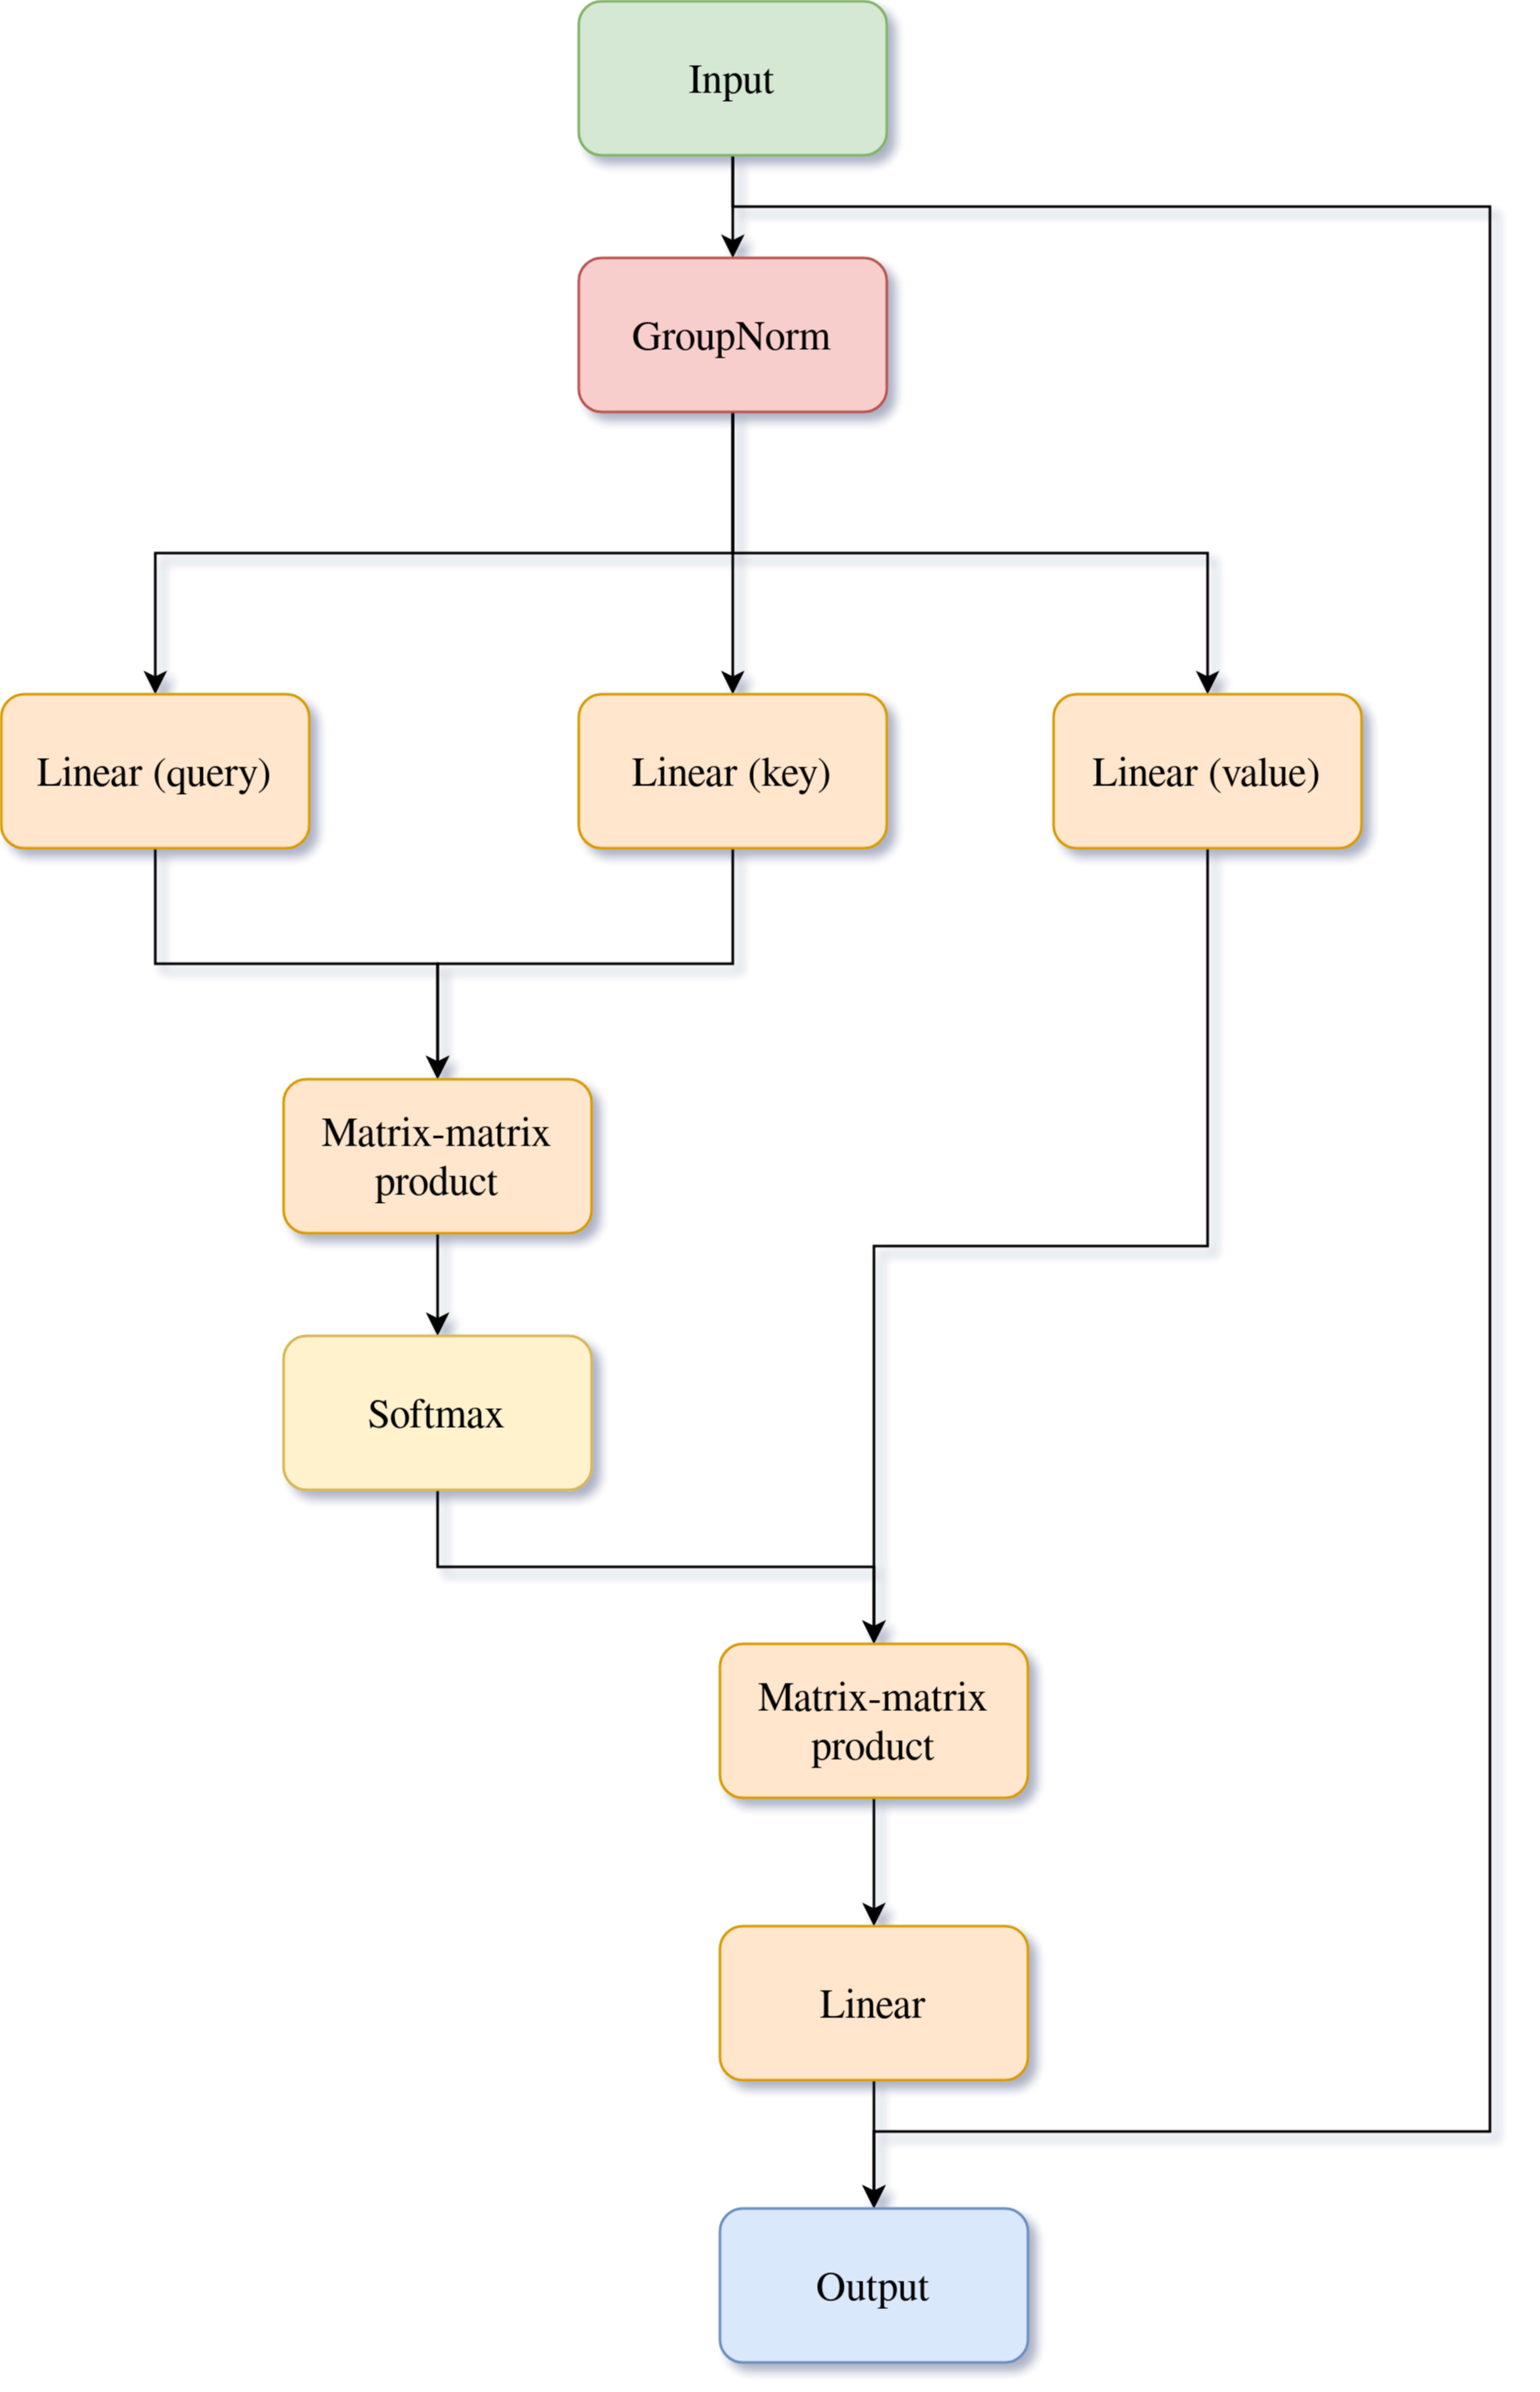
\includegraphics[scale=0.6]{images/AttentionBlock.drawio}
    \caption{Attention block architecture diagram}
\end{figure}

\subsection{Downsample and Upsample}
Downsample and upsample blocks are simple blocks that reduce or recover dimensions of input data and adjust number of channels. Using them we can obtain certain size of latent space.
\begin{figure}[H]
	\centering
	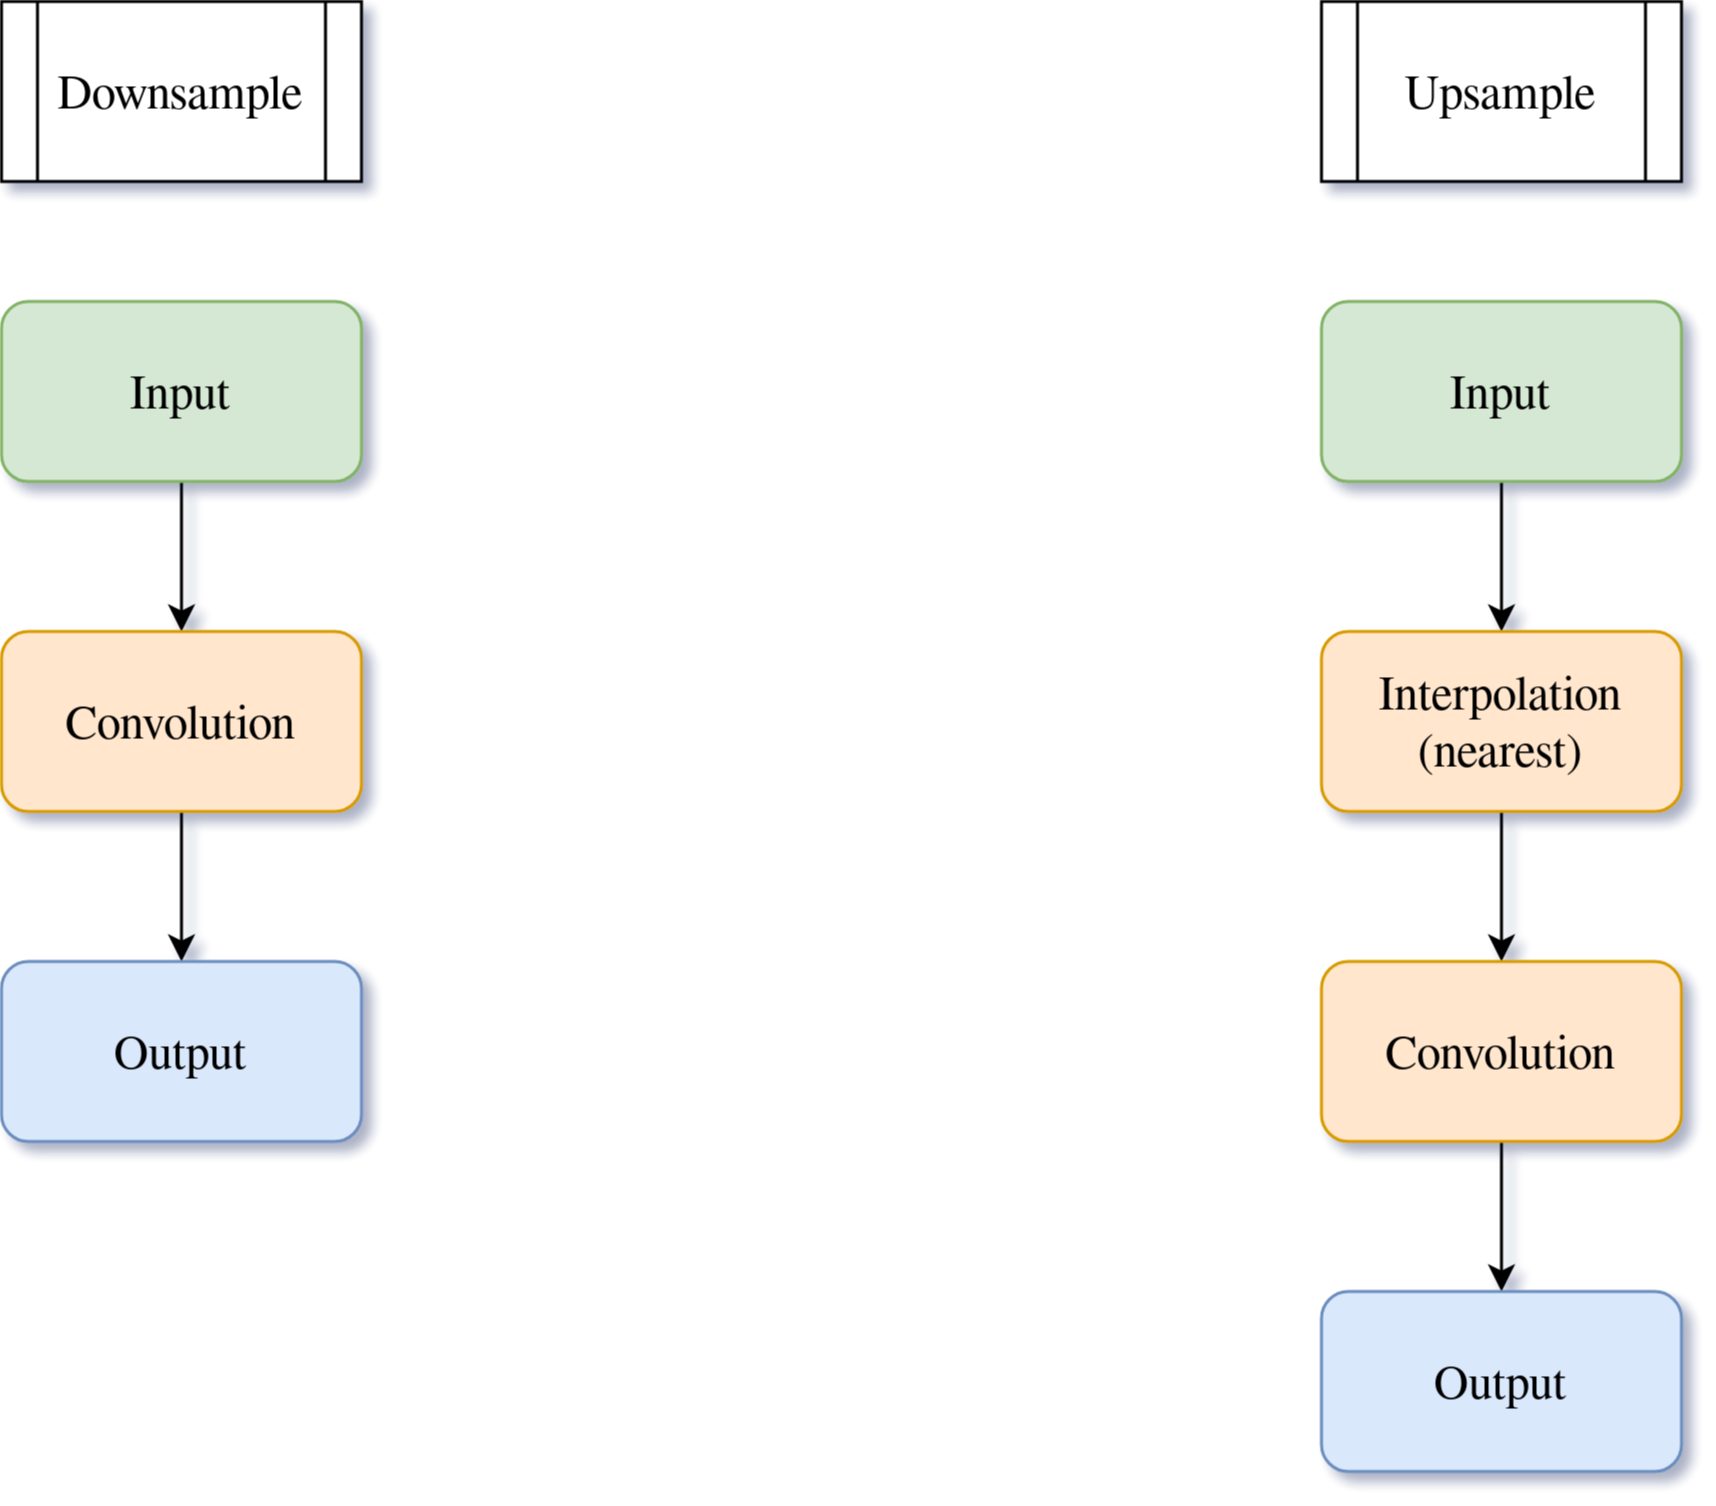
\includegraphics[scale=0.6]{images/UpDownSample.drawio}
    \caption{Downsample and upsample block architecture diagram}
\end{figure}

The modules above were used to build the more complex ones which are presented below. The modules below have two inputs or outputs depending on whether they are up or down. The output from the down blocks are directly connected with the input from up blocks.
\subsection{Resnet downsample and upsample}
These modules use resnet blocks and downsample or upsample blocks.
\begin{figure}[H]
	\centering
	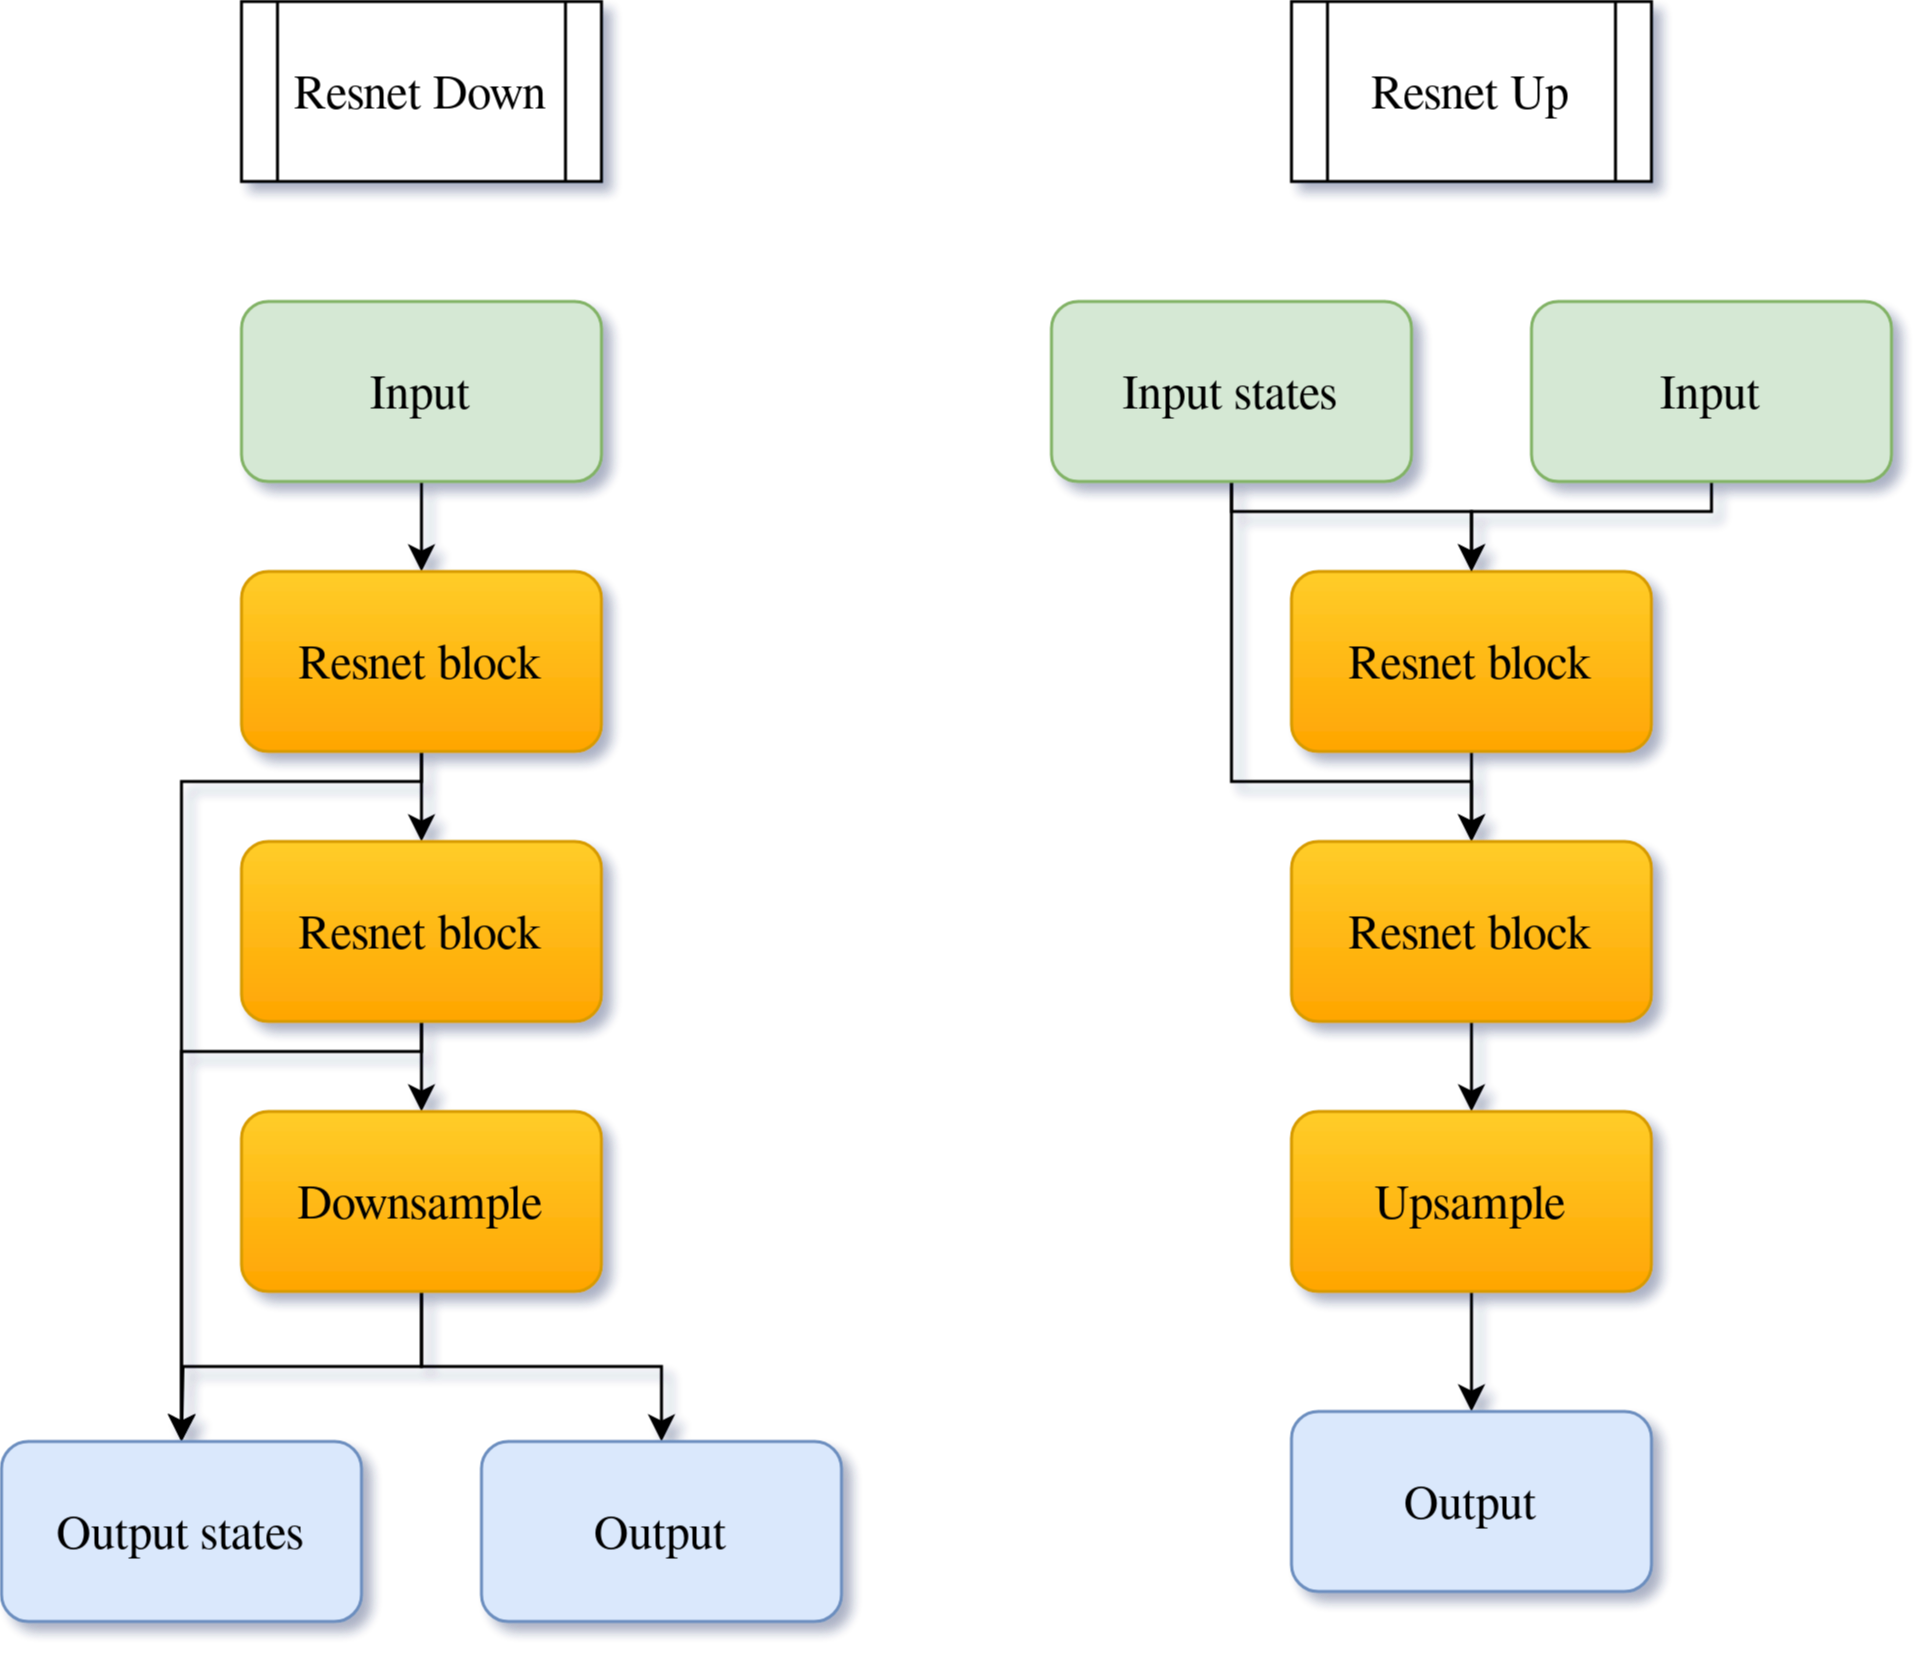
\includegraphics[scale=0.6]{images/ResnetDownUp.drawio}
    \caption{Restnet downsample and upsample block architecture diagram}
\end{figure}
\subsection{Attention downsample and upsample}
These modules are similar to downsample and upsambple but have additional attention blocks after every resnet blocks. 
\begin{figure}[H]
	\centering
	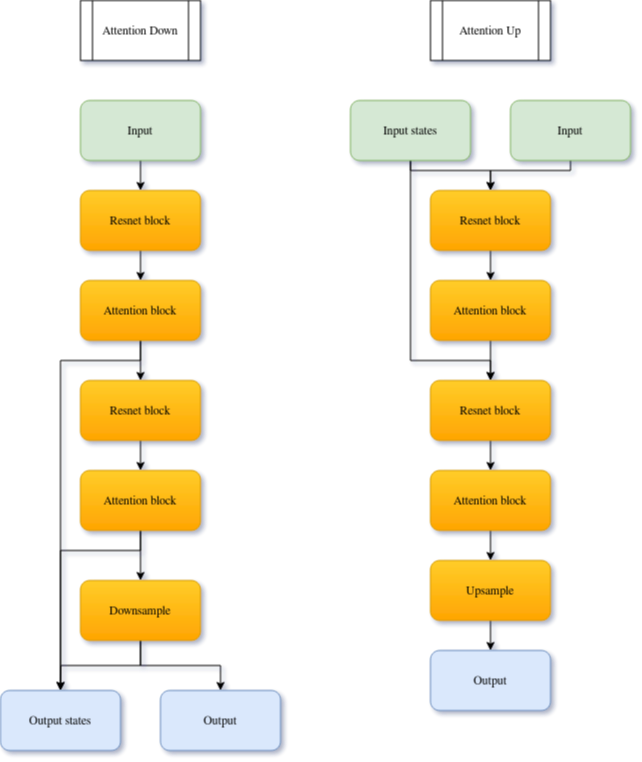
\includegraphics[scale=0.6]{images/AttentionDownUp.drawio}
    \caption{Attention downsample and upsample block architecture diagram}
\end{figure}

\subsection{Mid block}
Mid block is responsible for processing latent space. In this case latent space is not one dimensional so the resnet blocks with convolution are used, as well as attention block for learning the dependencies between individual parts of latent space.
\begin{figure}[H]
	\centering
	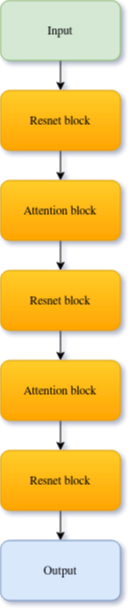
\includegraphics[scale=0.6]{images/MidBlock.drawio}
    \caption{Mid block architecture diagram}
\end{figure}

\subsection{Network architecture}
U-Net model is an architecture used in image generation. It has an encoder to capture features, a bottleneck for extraction, and a decoder for image generation. The model has additional skip connetions between encoder and decoder which help preserve fine details.
\begin{figure}[H]
	\centering
	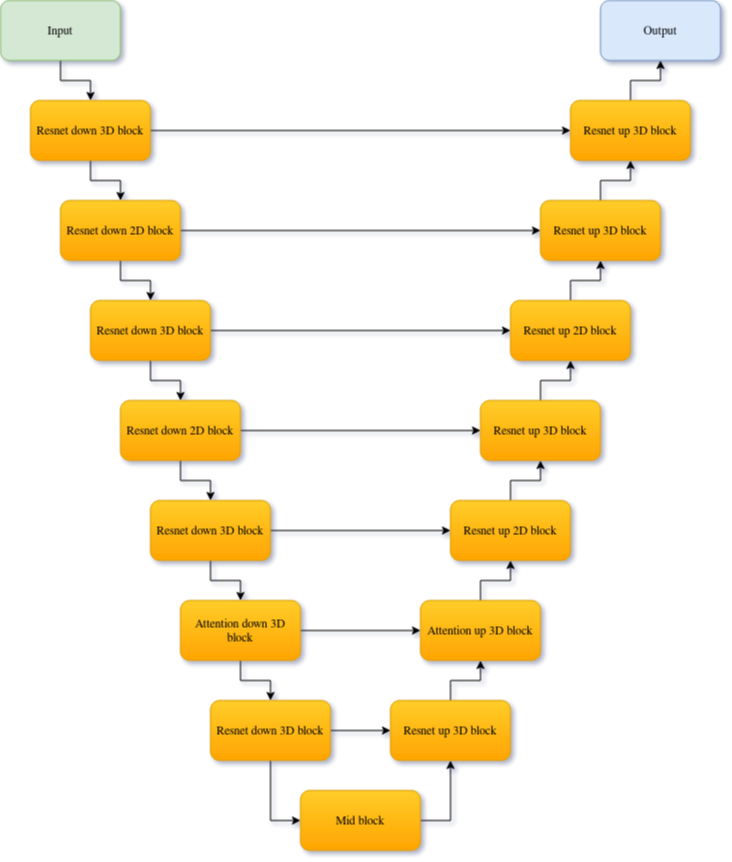
\includegraphics[scale=0.5]{images/ModelGraph.drawio}
    \caption{Network architecture}
\end{figure}
\subsection{Training parameters}
\subsubsection{Batch size}
In consideration of both the constraints posed by GPU memory limitations and the dataset's size, the decision was made to set the batch size to one.
\subsubsection{Learning rate}
A range of values, spanning from $10^{-7}$ to $3\cdot10^{-4}$, were systematically tested. It was observed that lower values within this range led to a slower learning pace and generated scans with considerably more noise. Conversely, as the values increased, the model's performance improved, with larger values yielding better results. However, it became evident that once the threshold of approximately $2\cdot10^{-4}$ was crossed, the model's stability during training became compromised, often becoming trapped in local minima.

In light of these findings, a careful evaluation led to the selection of the optimal value, which was determined to be $10^{-4}$. This value struck a balance between achieving satisfactory results and maintaining training stability, making it the most suitable choice.
\subsubsection{Number of epochs}
The number of epochs was established at 2000 due to the observation that the model's loss reached a plateau at this juncture, and further training did not yield any substantial improvements in results.


\section{Dataset}
The dataset contain a collection of 28 high-resolution computer tomography (CT) images that center on the prostate region. Each image has undergone meticulous hand-trimming to retain solely the pertinent anatomical features. This process results in a dataset that accentuates the vital elements essential for accurate interpretation.

These CT images grant a precise and detailed view of the prostate gland and its encompassing structures. The hand-trimming process has thoughtfully excluded irrelevant details and unrelated areas, leaving only a focused representation.

All images in this dataset adhere to a standardized dimension of 512 pixels by 512 pixels, presented across 26 individual slices. This 3D arrangement permits a comprehensive examination of the prostate from various perspectives and depths. The uniform image size and multiplicity of slices contribute to a thorough analysis and a more precise understanding of the prostate's configuration and potential discrepancies.

\begin{figure}[H]
	\centering
	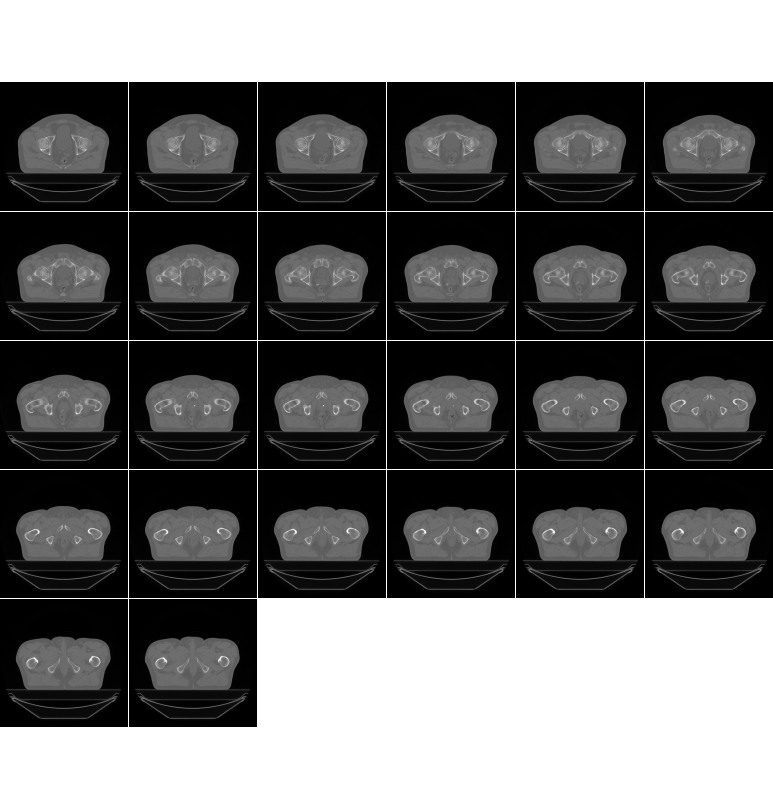
\includegraphics[scale=0.5]{images/datasetExample}
    \caption{Example from dataset}
\end{figure}
The dataset underwent a random partitioning procedure, resulting in the creation of two distinct subsets: a training dataset and a validation dataset. This division was executed in an 80-20 ratio, leading to a training subset comprising 23 images and a validation subset containing 5 images.

Furthermore, to enhance the dataset's diversity and training potential, augmentation techniques were applied. Random zoom and flilp operations were employed to augment the data. These augmentation methods introduce variations in scale and orientation, contributing to a more comprehensive and versatile dataset. The incorporation of such augmented data aids in training models that are better equipped to handle a wider range of real-world scenarios and variations.


\chapter{Results}
This chapter will present the outcomes study involving generative neural networks tasked with generating realistic CT scans. The aim of this investigation was to evaluate the network's ability to produce accurate and visually coherent medical images.

\section{Loss}
\begin{figure}[H]
	\centering
	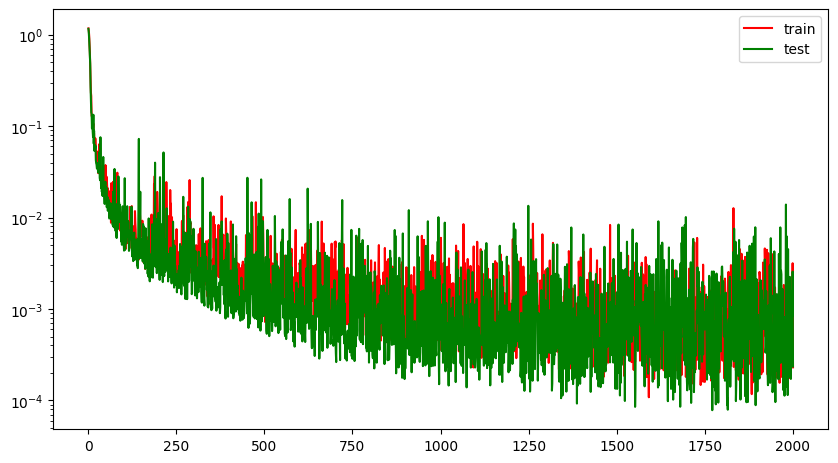
\includegraphics[scale=0.6]{images/loss}
    \caption{Loss history graph}
\end{figure}
Because of a relatively high learning rate, the graph shown above lacks clarity. To enhance its visibility, we calculate the average for every 10 epochs, resulting in a more visually accessible representation.
\begin{figure}[H]
	\centering
	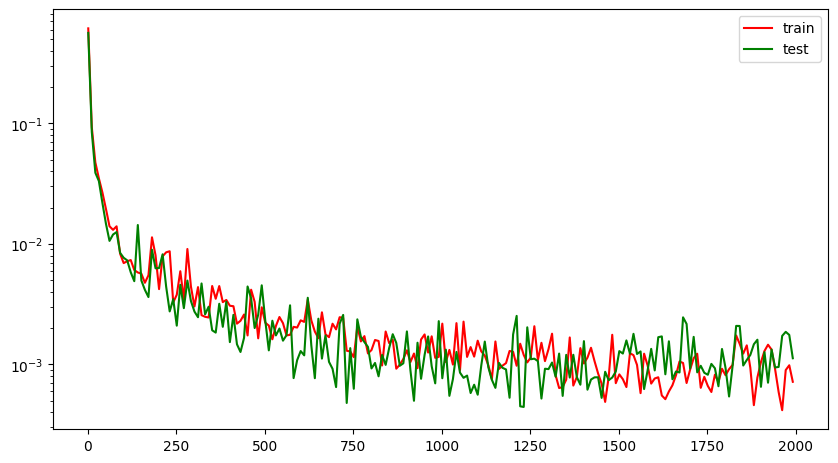
\includegraphics[scale=0.6]{images/loss_10}
    \caption{Average loss history graph}
\end{figure}
Both graphs utilize a logarithmic scale to display the training and test data loss. An observation drawn from these graphs suggests that the loss has reached a plateau, indicating that further training is unlikely to yield significant improvements in results.

\section{Generated CT scans}
\subsection{Examples}
\begin{figure}[H]
	\centering
	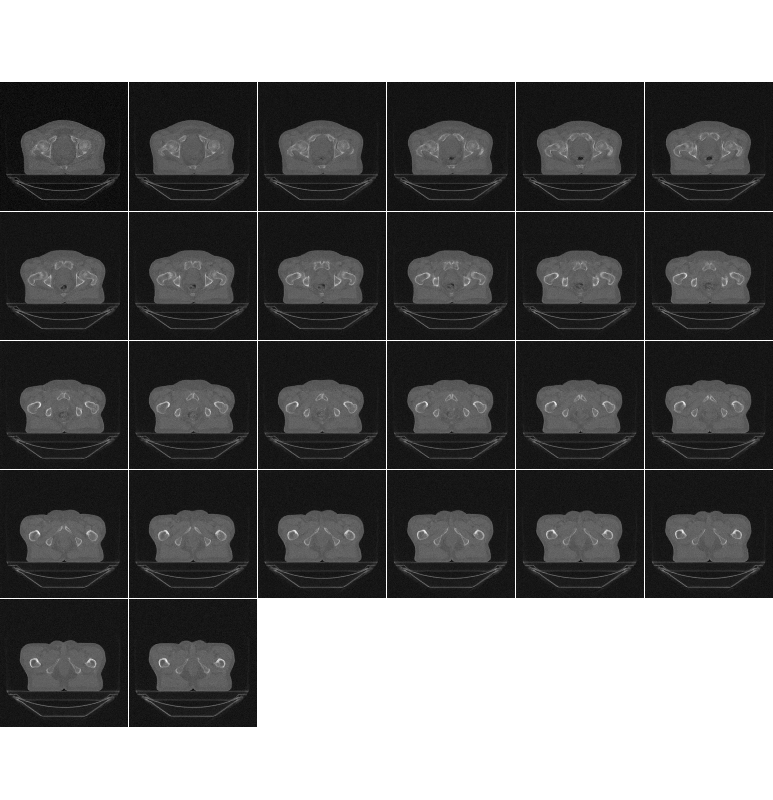
\includegraphics[scale=0.5]{images/generatedData1}
    \caption{CT scan generated by the model}
\end{figure}
\begin{figure}[H]
	\centering
	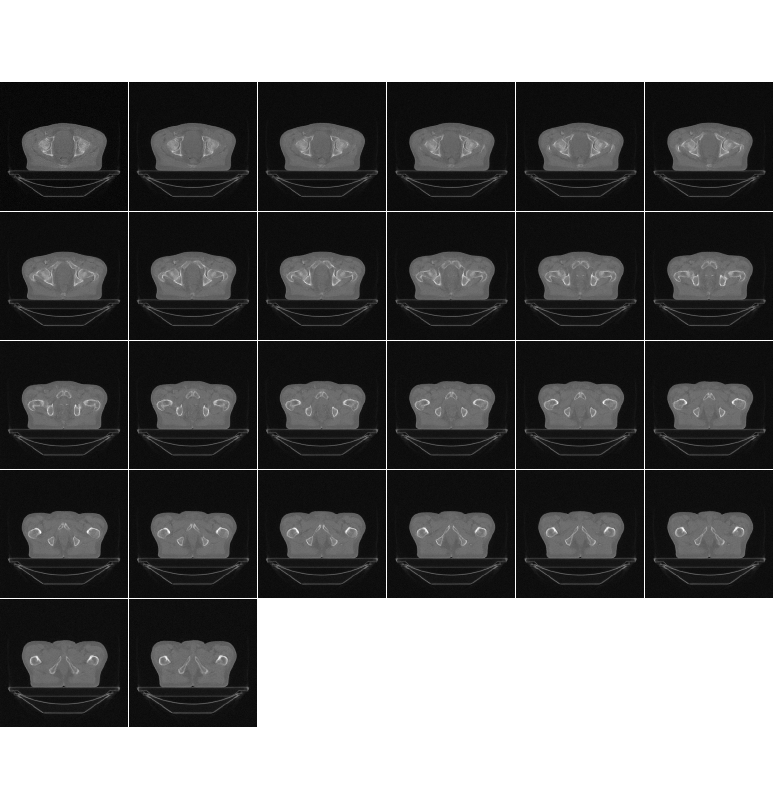
\includegraphics[scale=0.5]{images/generatedData2}
    \caption{CT scan generated by the model}
\end{figure}
\begin{figure}[H]
	\centering
	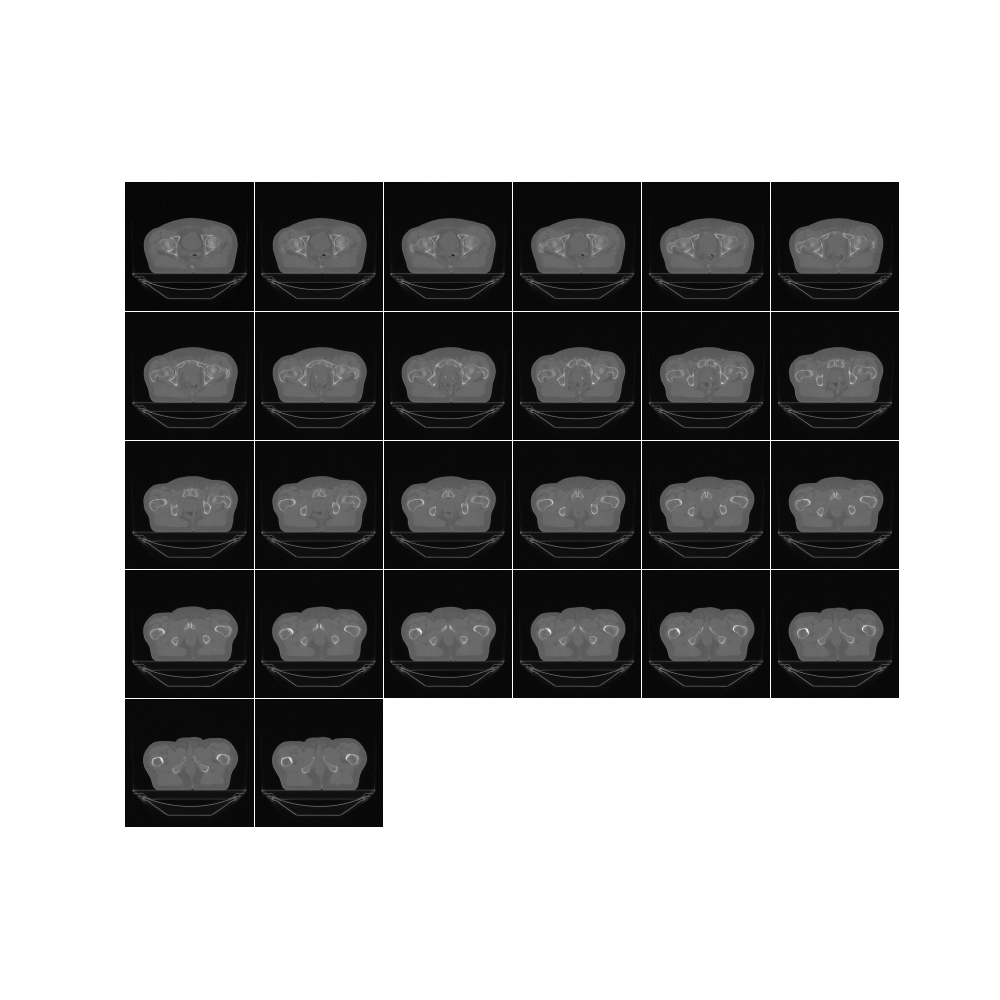
\includegraphics[scale=0.5]{images/generatedData3}
    \caption{CT scan generated by the model}
\end{figure}

\newpage
\subsection{Visual Realism and Quality}
Upon visual inspection, the generated CT scans exhibit a good level of realism and quality. Anatomical structures such as the prostate, bladder, and surrounding tissues are accurately portrayed, with textures and contrasts resembling those observed in actual CT scans. The model successfully captures the complex spatial relationships and proportions of anatomical structure.
\subsection{Variability and Diversity}
The network demonstrates proficiency in generating diverse images. It produces a spectrum of anatomical variations, encompassing different organ sizes, shapes, and orientations.
\subsection{Comparison to original data}
Comparing the generated CT images with their corresponding original counterparts reveals nuanced differences in various aspects. While the generated images bear a striking resemblance to the original CT scans in terms of anatomical structures and general features, there are certain distinctions worth noting. Notably, the generated CT images tend to exhibit slightly lower contrast levels in comparison to the originals, which could impact the visual clarity of certain structures. Additionally, a subtle increase in noise is observed in some of the generated images, which could potentially affect the interpretability of finer details. Furthermore, in some instances, the generated images may portray tissue textures that appear somewhat unnatural, suggesting room for improvement in capturing the intricate subtleties present in actual medical images.


\section{Limitations}

The current output of the model generates scans with a resolution of 256 by 256 pixels. However, it is important to note that this resolution is not enough to declare the generated samples have high quality. The limitation in resolution is primarily attributed to two key factors. First, there are constraints imposed by the available GPU memory, which dictates the practical upper limit for training process. Second, the underlying dataset itself has a resolution of 512 by 512 pixels. Consequently, the model is working within these constraints, resulting in the current resolution output.

Furthermore, it's worth emphasizing that evaluating the quality of these generated samples is a complex and require medical knowledge. The intricacies of medical imaging might only be evident to experts.
\section{Future Directions}
The next logical move would be to attempt generating higher-resolution samples by using multiple GPUs.

Future research endeavors could explore refining the network architecture for enhanced in image quality and anatomical accuracy. Expanding the study to larger datasets could further enrich the generative capabilities. Additionally, the model can be trained on datasets with different organs to check the performance in slightly different task.

\addcontentsline{toc}{chapter}{\protect\numberline{}Bibliographic}
\begin{thebibliography}{99}

% TODO data of access???
\bibitem{DDPM}
\url{https://arxiv.org/pdf/2006.11239.pdf}

\bibitem{ImprovedDDPM}
\url{https://arxiv.org/pdf/2102.09672.pdf}

\bibitem{diffBeatGan}
\url{https://arxiv.org/pdf/2105.05233.pdf}

\bibitem{HighResImageSyntesis}
\url{https://arxiv.org/pdf/2112.10752.pdf}

\bibitem{TextToImage}
\url{https://arxiv.org/pdf/2205.11487.pdf}
  
\bibitem{lw_diffusion}
\url{ https://lilianweng.github.io/posts/2021-07-11-diffusion-models/}

\bibitem{jalammar_diffusion}
\url{http://jalammar.github.io/illustrated-stable-diffusion/}

\bibitem{vaeLogLikelihhod}
\url{https://arxiv.org/pdf/2206.09453.pdf}

\bibitem{diffusionWiki}
\url{https://en.wikipedia.org/wiki/Diffusion_model}

\bibitem{vaeWiki}
\url{https://en.wikipedia.org/wiki/Variational_autoencoder}

\bibitem{unetSegmentation}
\url{https://arxiv.org/pdf/1505.04597v1.pdf}

\bibitem{unetWiki}
\url{https://en.wikipedia.org/wiki/U-Net}

\bibitem{stableDiffusionGithub}
\url{https://github.com/CompVis/stable-diffusion}

\bibitem{latentDiffModel}
\url{https://ommer-lab.com/research/latent-diffusion-models/}

\bibitem{convolution}
Ian Goodfellow and Yoshua Bengio and Aaron Courville, Deep Learning, 2015
\url{https://www.deeplearningbook.org/}

\bibitem{AttentionIsAll}
\url{https://arxiv.org/pdf/1706.03762.pdf}

\bibitem{AttentionWiki}
\url{https://en.wikipedia.org/wiki/Attention_(machine_learning)}

\bibitem{TransformersWiki}
\url{https://w.wiki/7MW8}

\bibitem{Michal}
Analysis of the quality of CT medical data generation using a pre-trained GAN model, Michał Orlewski, 2023

\bibitem{Python}
\url{https://www.python.org/}

\bibitem{Pytorch}
\url{https://pytorch.org/}

\bibitem{Monai}
\url{https://monai.io/}
  
\bibitem{Hf_diffusers}
\url{https://huggingface.co/docs/diffusers/index}

\bibitem{Hf_diffusers_gh}
\url{https://github.com/huggingface/diffusers}

\bibitem{Resnet}
\url{https://en.wikipedia.org/wiki/Residual_neural_network}

\bibitem{PytorchDoc}
\url{https://pytorch.org/docs/stable/index.html}
  
\end{thebibliography}
\end{document}
